% Copyright (c) 2020-2025 Simon Crase

% Permission is hereby granted, free of charge, to any person obtaining a copy
% of this software and associated documentation files (the "Software"), to deal
% in the Software without restriction, including without limitation the rights
% to use, copy, modify, merge, publish, distribute, sublicense, and/or sell
% copies of the Software, and to permit persons to whom the Software is
% furnished to do so, subject to the following conditions:

% The above copyright notice and this permission notice shall be included in all
% copies or substantial portions of the Software.

% THE SOFTWARE IS PROVIDED "AS IS", WITHOUT WARRANTY OF ANY KIND, EXPRESS OR
% IMPLIED, INCLUDING BUT NOT LIMITED TO THE WARRANTIES OF MERCHANTABILITY,
% FITNESS FOR A PARTICULAR PURPOSE AND NONINFRINGEMENT. IN NO EVENT SHALL THE
% AUTHORS OR COPYRIGHT HOLDERS BE LIABLE FOR ANY CLAIM, DAMAGES OR OTHER
% LIABILITY, WHETHER IN AN ACTION OF CONTRACT, TORT OR OTHERWISE, ARISING FROM,
% OUT OF OR IN CONNECTION WITH THE SOFTWARE OR THE USE OR OTHER DEALINGS IN THE
% SOFTWARE.

\documentclass[]{article}
\usepackage{float}
\usepackage{url}
\usepackage{amsmath}
\usepackage{graphicx}
\graphicspath{{./figs/}}

%opening
\title{An Agent Based Model to study stability of Ecosystems: Proposal}
\author{Simon Crase}

\begin{document}

\maketitle

\begin{abstract}
The Grass/Sheep/Wolves model \cite{Wilensky:1997,wilensky2006thinking} exhibits behaviour that I did not expect: it appeared stable with the default values of parameters, but when I increased the speed at which grass regrows slightly, regrowth time=20, the model ran for some 1,200,000 generations, the wolves become extinct suddenly--Figure \ref{fig:wsg}. It is not clear whether this is a limitation of the simple model.  The proposed model seeks to establish whether the well known link between diversity and stability emerges from simple dynamics.
\end{abstract}

\begin{figure}[b]
	\centering
	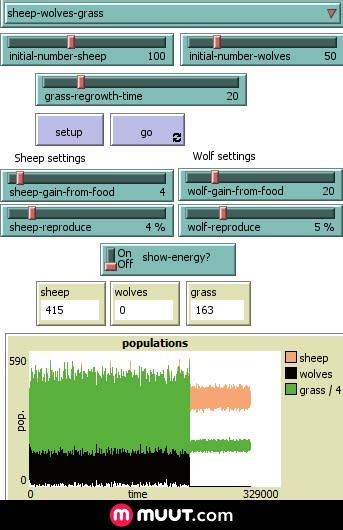
\includegraphics[width=0.5\linewidth]{wsg20.jpg}
	\caption{Wolves Sheep Grass. This run crashes after a couple of hundres thousand generations, but I have observed over 1,200,000. Notice that the crash is very sudden, and that the grass, and presumably the sheep, move through a smaller range after the crash.}
	\label{fig:wsg}
\end{figure}

\section{What part of phenomenon would you like to model?}

I would like to understand the relationship between species diversity and stability in a simulated ecology with Natural Selection. Although it is well accpeted that diversity is correlated with stability, e.g. \cite{cleland:2011}, I would like to see whether this emerges directly from a simulation of behaviour of individuals. I plan to make the simulation asexual initially, to avoid the complexities of Mendelian inheritance.

\section{What are the principal types of agents involved in this phenomenon?}

\begin{enumerate}
	\item Primary producers
	\item Consumers. There may be multiple species in each level.
	\begin{enumerate}
		\item Primary
		\item Secondary
		\item Tertiary 
	\end{enumerate}
\end{enumerate}

\section{What properties do these agents have?}

\begin{enumerate}
	\item Primary producers
	\begin{enumerate}
		\item Energy
	\end{enumerate}
	\item Consumers
	\begin{enumerate}
		\item Energy
		\item speed
		
	\end{enumerate}
\end{enumerate}

\section{What actions (or behaviours) can these agents take?}

\begin{enumerate}
	\item Primary producers
	\begin{enumerate}
		\item Grow--acquire energy at a uniform rate
		\item Be eaten--lose energy to a Consumer
	\end{enumerate}	
	\item Consumers
	\begin{enumerate}
		\item Breed--transfer some energy to offspring; this is less than 100\% efficient, so the cost of breeding exceeds the total energy transferred. 
		\item Wander/pursue--expend energy in source of food.
		\item Feed--acquire energy from a producer or lower level consumer; energy gained is less than that lost by the food source.
		\item Die--when energy is depleted, or after a certain number of generations.
		\item Mutate--when offspring are created, some parameters may be changed, e.g. pursuit speed, number of offspring, energy per offspring. I expect this to optimize the parameters to maximize inclusive fitness \cite{wiki:inclusive}.
	\end{enumerate}
\end{enumerate}


\section{If the agents have goals, what are their goals?}

\begin{enumerate}
	\item Live as long as possible
	\item Make as many copies of itself as possible
\end{enumerate}

\section{Agents operate in what kind of environment?}

I envisage a collection of patches that represent primary producers; consumers move around, either randomly or purposefully moving towards food.   

\section{How do agents interact with environment?}

\begin{enumerate}
	\item Consumers move around, which costs energy, and drive energy from the environment (primary consumers), or from lower level consumers.
	\item Consumers can breed if they have enough energy to pay the cost; children get a portion of the parent's energy. We'll make it asexual to start with.
	
\end{enumerate}

\section{What do I hope to observe}

Some evidence that more species at start $\implies$ a longer time before population crashes.

\medskip

\bibliographystyle{unsrt}
\bibliography{../complexity}

\end{document}
